\documentclass{article}
% s e l e c c i o n a e l t i p o de documento
\usepackage[spanish]{babel}
%
\usepackage[T1]{fontenc}
\usepackage[latin1]{inputenc}
\usepackage{graphicx}
\begin{document}
% i n i c i o d e l cuerpo d e l documento
\title{Laboratorio 1}
\author{Jean Carlos Chavarr\' ia Hughes B11814}
\maketitle
% t i t u l o d e l documento
\begin{abstract}
Laboratorio 4 de el curso IE 0217.
\end{abstract}
\section{Introducci\' on}
Este documento corresponde al reporte de cuarto laboratorio del curso IE0217, en el cual se trabaj\' o con distintos tipos de estructuras de datos de de C++, espec\' ificamente \textbf{queue} y \textbf{stack}. 
Adem\' as se trabaj\' o tambien creando clases y con las caracter\' isticas de \textbf{herencia}.

\section{Comentarios Importantes}

\subsection{Porqu\' e mi$\_$figura puede usarse para direccionar mi$\_$circulo si son de tipos diferentes}

Se puede recordar que en C++ y en cualquier lenguaje de programacion en general, las clases son tipos. Tipos de datos definidos por el usuario y como tal pueden ser apuntandos por punteros.  Ahora, el puntero \textbf{mi$\_$figura} se puede usar para direccionar el objecto \textbf{mi$\_$circulo} aunque son tipos diferentes, pero debido a la herencia que recibo \textbf{mi$\_$circulo} proveniente de la clase madre, se puede entender como del mismo tipo o familia de datos.

\subsection{Edite el archivo figura.h e incluya la palabra virtual antes de la declaraci\' on de la funci\' on mover, recompile todo y ejecute de nuevo el programa}

A la hora de compilar no apareci\' o ning\' un problema, y cuando se ejecut\' o el ejecutable \textbf{principal}  el resultado desplegado fue exactamente el mismo en consola.

Sin embargo hay diferencias con el uso y el desuso de la directiva \textbf{virtual}.

Sin el uso de \textbf{virtual} se obtiene una conexi\' on temprano, la cual se refiere a que la implementaci\' on del m\' etodo que se llama se realiza en tiempo de compilaci\' on, basado en el tipo de puntero que se llama.

Con el uso de \textbf{virtual} se obtiene una conexi\' on tard\' ia, lo cual se refiere a que la implementaci\' on del m\' etodo que se llama se realiza en tiempo de ejecuci\' on, basado en el tipo de puntero que fue originalmente construido.



\subsection{Estructuras de datos}
Para la parte del laboratorio relacionada con la cola y la pila se requiri\' o mucho m\' as tiempo debido a que esta relacionado con el manejo de punteros y estructuras de datos que a\' un no se conocian.

En t\' erminos generales, en el que se relaciona con la cola o \textbf{queue}, utiliza dos punteros, \textbf{first} y \textbf{last}, los cuales se manejan de manera que cuando se crean nuevos \textbf{nodos}, se manipula para que de nuevo el puntero last apunte al nuevo ultimo elemento y first al primero. 

Para que sea m\' as sencillo de visualizar se puede observar la Figura \ref{fig:principalqueue} y \ref{principalstack}.

\begin{figure}[H]
\caption{Principal Queue}
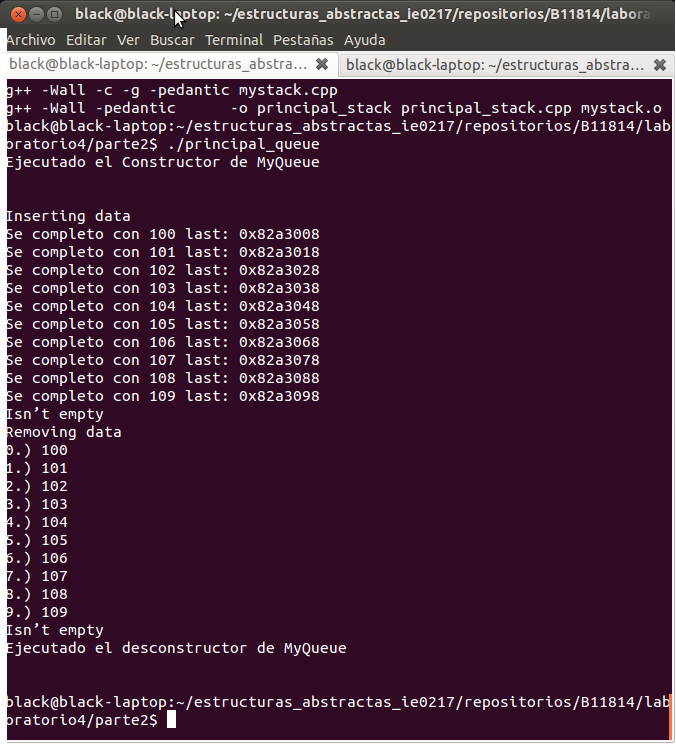
\includegraphics[scale=0.6]{./imagenes/principalqueue.png}
\label{fig:principalqueue}
\end{figure}

\begin{figure}[H]
\caption{Principal Queue}
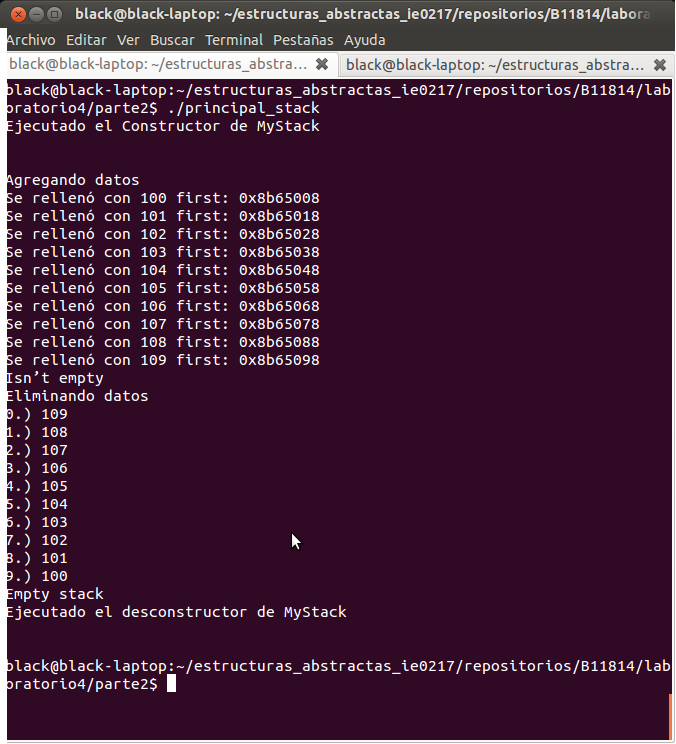
\includegraphics[scale=0.6]{./imagenes/principalstack.png}
\label{fig:principalstack}
\end{figure}




\end{document}
